\documentclass[a4paper,10pt]{article}
\usepackage[a4paper, left=3cm,right=2.5cm]{geometry}

\usepackage[spanish]{babel}
\selectlanguage{spanish}
\usepackage[utf8]{inputenc}
\usepackage[pdftex]{graphicx}

% Utilizado para recuadrar expresiones
\usepackage{amsmath}
% Recuadros con mayor separación
\setlength{\fboxsep}{6pt}

\def \anio {a\tilde{n}o}

\begin{document}

\paragraph{Ejercicio 1} A continuación se presenta la red, con el camino crítico resaltado en trazo grueso; esta comprende las actividades B, C, D, E y J. La duración del proyecto es de 23 semanas.

    \begin{center}
	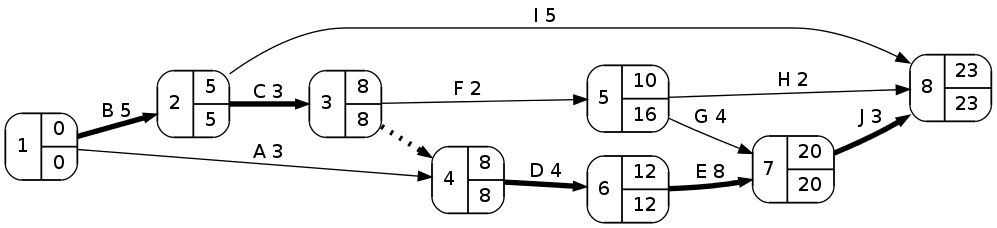
\includegraphics[scale=0.55,keepaspectratio=true]{img/ej1-red.png} 
	\end{center}
  
\end{document}
